\documentclass[conference]{IEEEtran}
\IEEEoverridecommandlockouts
\usepackage{cite}
\usepackage{amsmath,amssymb,amsfonts}
\usepackage{algorithmic}
\usepackage{graphicx}
\usepackage{textcomp}
\usepackage{xcolor}
\usepackage{hyperref}
\def\BibTeX{{\rm B\kern-.05em{\sc i\kern-.025em b}\kern-.08em
    T\kern-.1667em\lower.7ex\hbox{E}\kern-.125emX}}
\begin{document}

%%%%%%%%%%%%%%%%%%%%%%%%%%%%%%%%%%%%%%%%%%%%%%%%%%%%%%%%%%%%%%%%%%%%%%%%%%%%%%%%%%
\title{
    HYDRA: High-Yield Data Reorganization \& Acceleration\\
    \large Final Report \\
}
%%%%%%%%%%%%%%%%%%%%%%%%%%%%%%%%%%%%%%%%%%%%
\author{
    \IEEEauthorblockN{
        Nafil Atiq\IEEEauthorrefmark{1},
        Ruohan Dong\IEEEauthorrefmark{1},
        Matthew Nutt\IEEEauthorrefmark{1},
        Giovanni Sirtori\IEEEauthorrefmark{1},
        Ithzel Toscano\IEEEauthorrefmark{1},
        Yulia Zhou\IEEEauthorrefmark{1}
}
%%%%%%%%%%%%%%%%%%%%%%%%%%%%%%%%%%%%%%%%%%%%
\IEEEauthorblockA{
    \IEEEauthorrefmark{1}%
    Department of Electrical \& Computer Engineering \\
    Rice University, Houston, Texas \\
    \{na115, rd100, mcn5, gs86, ijt2, yz305\}@rice.edu}
}
%%%%%%%%%%%%%%%%%%%%%%%%%%%%%%%%%%%%%%%%%%%%
\maketitle
%%%%%%%%%%%%%%%%%%%%%%%%%%%%%%%%%%%%%%%%%%%%%%%%%%%%%%%%%%%%%%%%%%%%%%%%%%%%%%%%%%
\begin{abstract}
    Modern AI inference on embedded RISC-V processors is throttled by 
    data-movement operations --- matrix transpositions, quantization, and 
    non-contiguous gathers --- which consume CPU cycles and pollute the L1 
    cache without contributing to arithmetic throughput. This report 
    presents HYDRA (High-Yield Data Reorganization \& Acceleration), a 
    smart-DMA engine designed as a second AHB-Lite master in the CORE-V 
    Wally RISC-V SoC. HYDRA defines three transformation modes: 
    scatter-gather (Mode~A), 8$\times$16 ping-pong-buffered matrix 
    transposition with an early-drain optimization (Mode~B), and 
    combinational INT32-to-INT8 quantization with 4:1 packing (Mode~C). 
    Modes~B and~C are implemented in synthesizable SystemVerilog and 
    verified in simulation. In parallel, the team developed a UVM-based 
    verification flow for the data cache and core, and a scan-based DFT 
    framework that improved fault coverage from 52\% to 71\%. Full SoC 
    integration and performance characterization are the next milestones.
\end{abstract}
%%%%%%%%%%%%%%%%%%%%%%%%%%%%%%%%%%%%%%%%%%%%%%%%%%%%%%%%%%%%%%%%%%%%%%%%%%%%%%%%%%
\begin{IEEEkeywords}
    RISC-V, DMA, RTL, UVM, SystemVerilog, AHB-Lite, quantization
\end{IEEEkeywords}
%%%%%%%%%%%%%%%%%%%%%%%%%%%%%%%%%%%%%%%%%%%%%%%%%%%%%%%%%%%%%%%%%%%%%%%%%%%%%%%%%%
\section{Introduction}
    Modern AI inference systems are increasingly bottlenecked by irregular 
    memory access patterns in operations such as embedding lookup, sparse 
    attention, and tensor layout conversion~\cite{tripp2024}. Traditional 
    DMA engines like the TI EDMA~\cite{ti_edma} improve raw bandwidth but 
    lack semantic awareness, while full ML accelerators are costly and 
    inflexible. We present HYDRA (High-Yield Data Reorganization \& 
    Acceleration), a programmable DMA engine with an AI-aware datapath 
    that performs in-flight transformations. HYDRA implements three 
    hardware-accelerated modes: scatter-gather for irregular access prefetch 
    (Mode~A), corner-turning for matrix transpose (Mode~B), and real-time 
    quantization to multiply effective bandwidth (Mode~C). The engine 
    integrates into the CORE-V Wally RISC-V SoC~\cite{harris2022wally}, 
    inheriting its verified L1 cache and AHB-Lite bus infrastructure. 
    This report covers the team's work across RTL design and SoC integration 
    on Wally, alongside DFT and UVM verification frameworks developed on 
    an earlier RISC-V core that will be ported to Wally next semester.
%%%%%%%%%%%%%%%%%%%%%%%%%%%%%%%%%%%%%%%%%%%%%%%%%%%%%%%%%%%%%%%%%%%%%%%%%%%%%%%%%%
\section{Methods}
%%%%%%%%%%%%%%%%%%%%%%%%%%%%%%%%%%%%%%%%%%%%
    \subsection{RTL Design and SoC Integration}
        HYDRA is implemented as a second AHB-Lite bus master in the Wally SoC, 
        peer to the CPU's External Bus Unit, following the modular front-end / 
        mid-end / back-end DMA decomposition of Benz et al.~\cite{benz2023}. 
        \texttt{hydra\_mmr.sv} implements the AHB slave register file (front-end), 
        exposing CTRL, SRC, DST, LEN, MODE, and STATUS registers to the CPU. 
        \texttt{hydra\_transform.sv} contains the address generation unit and 
        the transformation datapath (mid-end), together with the AHB master 
        state machine that issues burst transactions on the data plane (back-end). 
        \texttt{hydra\_arbiter.sv} mediates bus contention between HYDRA and 
        the CPU through a Moore FSM with a registered grant output, breaking 
        any combinational path from \texttt{HBUSREQ} to \texttt{HADDR}. 
        \texttt{hydra\_scratchpad.sv} provides a dual-port memory: an AHB-Lite 
        slave port for CPU reads and a private sideband write port for HYDRA. 
        This decoupling is essential --- routing HYDRA's writes through the AHB 
        fabric would serialize them with its read transactions, eliminating 
        the fill/drain overlap that Mode~B's ping-pong design relies on. The 
        full topology is shown in Fig.~\ref{fig:hydra-block}.
        
        \begin{figure}[h]
        \centering
        \fbox{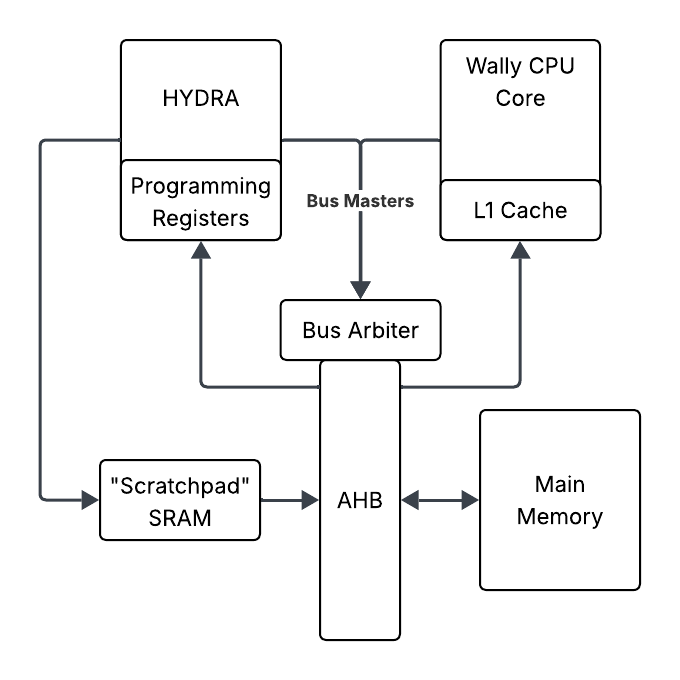
\includegraphics[width=0.8\linewidth]{figures/HYDRA_diag.png}}
        \caption{Full system block diagram.}
        \label{fig:hydra-block}
        \end{figure}
        
        Mode~B (Corner-Turning) partitions the source matrix into $8 \times 16$ 
        blocks of 32-bit words, exactly matching one Wally cache line per row, following the block corner-turning method of Ma et al.~\cite{ma2019}. 
        Two ping-pong SRAM buffers operate concurrently: one drains column-major 
        to the scratchpad while the other fills row-major from main RAM. An 
        early-drain optimization further reduces per-block latency by exploiting 
        the row-major-fill / column-major-drain index skew. Drain can begin on 
        the same buffer still being filled provided the fill counter leads the 
        drain counter by at least $(N-1)(M-1) = 105$ beats, saving 22 of the 
        128 cycles otherwise spent waiting for the first buffer to complete 
        before standard ping-pong overlap takes over.
        
        Mode~C implements a fully combinational rounding-and-saturation pipeline 
        (\texttt{quant\_fn} in \texttt{hydra\_pkg.sv}) that converts INT32 inputs 
        to INT8 outputs and packs four results into each 32-bit bus word, 
        multiplying effective destination bandwidth by 4$\times$ per 
        Equation~\ref{eq:bw}. The quantization unit is configurable at runtime 
        through MMR fields for scale shift, signed/unsigned output, and 
        rounding-mode enable, allowing the same hardware to serve audio (signed) 
        and image (unsigned) workloads.
        
        \begin{equation}
        B_{\text{eff}} = B_{\text{raw}} \times \frac{W_{\text{src}}}{W_{\text{dst}}}
        \label{eq:bw}
        \end{equation}
        
        Cache coherency is resolved by construction through the memory map in 
        Table~\ref{tab:memmap}: HYDRA writes only to the non-cacheable scratchpad 
        region (\texttt{0x2001\_0000}), so no line ever needs invalidation and 
        no \texttt{fence.i} is required from software. The MMR slave is 
        zero-wait-state, with \texttt{HREADYOUT} permanently asserted. Wally 
        is integrated as a Git submodule with patches applied through a 
        reproducible script workflow, keeping the HYDRA repository lightweight 
        and version-agnostic across Wally upstream changes.
        
        \begin{table}[h]
        \caption{HYDRA SoC Memory Map}
        \label{tab:memmap}
        \centering
        \begin{tabular}{llll}
        \hline
        \textbf{Region} & \textbf{Base Address} & \textbf{Size} & \textbf{Attribute} \\
        \hline
            Boot ROM         & \texttt{0x0000\_1000} & 4 KB   & Read-only \\
            CLINT            & \texttt{0x0200\_0000} & 64 KB  & MMIO \\
            PLIC             & \texttt{0x0C00\_0000} & 64 MB  & MMIO \\
            UART / GPIO      & \texttt{0x1000\_0000} & --     & MMIO \\
            HYDRA MMR        & \texttt{0x2000\_0000} & 4 KB   & Non-cacheable \\
            Scratchpad SRAM  & \texttt{0x2001\_0000} & 4 MB   & Non-cacheable \\
            Main RAM         & \texttt{0x8000\_0000} & 128 MB & Cached (I\$/D\$) \\
        \hline
        \end{tabular}
        \end{table}
%%%%%%%%%%%%%%%%%%%%%%%%%%%%%%%%%%%%%%%%%%%%
    \subsection{Design for Testability (DFT)}
        I first built a lightweight scan-based ATPG framework at the RTL level, including pattern generation, scan control, and fault evaluation as shown in Fig.~\ref{fig:DFT Architecture.png}. 
        
        \begin{figure}[h]
            \centering
            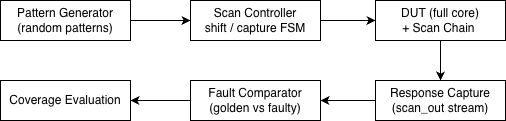
\includegraphics[width=1.0\linewidth]{figures/DFT_arch.png}
            \caption{Scan-based ATPG framework}
            \label{fig:DFT Architecture.png}
        \end{figure}
        
        Using this framework, I first obtained a baseline fault coverage of approximately 52.31\%, I performed a more detailed analysis by separating the results across different pipeline stages. This breakdown revealed that the coverage of pipeline reg3 was significantly lower than that of pipeline reg0, reg1, and reg2.
        
        Based on this observation, I focused on pipeline reg3 and designed a targeted test to investigate its testability. I injected faults into specific bits of the scan chain corresponding to pipeReg3 and monitored both the register value and its functional input during the capture cycle. Key signals such as \texttt{enable\_design}, \texttt{scan\_en}, and internal data paths were observed to determine whether the injected faults could propagate and become observable.
        
        \begin{figure}[h]
            \centering
            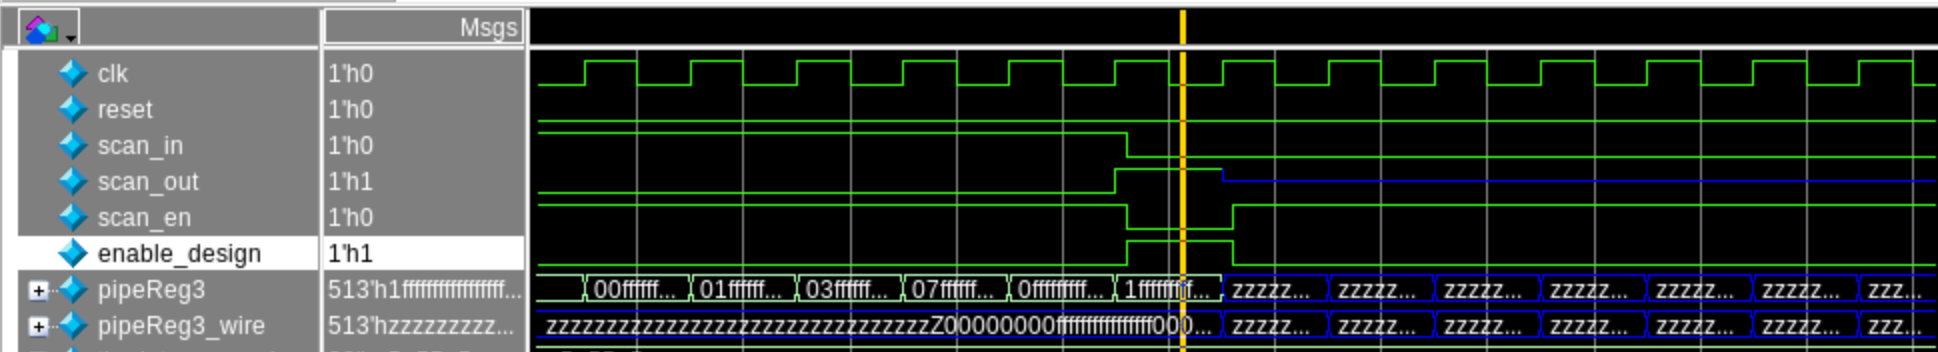
\includegraphics[width=1.0\linewidth]{figures/DFT_pipe.png}
            \caption{Waveform showing fault behavior in pipeReg3}
        \end{figure}
        
        As shown, pipeReg3 is correctly loaded with the injected fault during the shift-in phase. However, when the design enters the capture phase (indicated by \texttt{enable\_design = 1}), the register value is overwritten by its functional input (pipeReg3\_wire). As a result, the injected fault is eliminated before it can propagate to observable outputs.
        
        Based on this finding, I conclude that pipeline reg3 has inherently low observability under the current testing methodology. Therefore, instead of further optimizing reg3, I focus on improving the coverage of pipeline reg0, reg1, and reg2 using enhanced testing strategies.
%%%%%%%%%%%%%%%%%%%%%%%%%%%%%%%%%%%%%%%%%%%%
    \subsection{Data Cache Verification Framework}
        This work adopts a UVM-based verification methodology to validate a direct-mapped data cache. The DUT is a 2 KB cache with 32-byte cache lines, implementing a write-through and no-write-allocate policy.
        
        A layered UVM architecture is constructed, consisting of a test, environment, agent, and scoreboard. The environment contains a CPU agent, which includes a sequencer, driver, and monitor. The sequencer generates transaction-level stimuli, the driver translates them into pin-level signals through a SystemVerilog interface, and the monitor reconstructs transactions from DUT outputs.
        
        A scoreboard with an integrated reference model is used for functional checking. The reference model maintains expected memory behavior and cache semantics, enabling automatic comparison between expected and observed results on a per-transaction basis.
        Stimulus generation follows a constrained-random strategy with 200 transactions per run. To ensure sufficient coverage of cache behaviors, a biased distribution is applied: 70\% address reuse to generate cache hits, and 30\% new addresses to trigger cache misses. Read and write operations are randomly interleaved to cover all combinations of hit/miss scenarios.
%%%%%%%%%%%%%%%%%%%%%%%%%%%%%%%%%%%%%%%%%%%%
    \subsection{Core Verification Framework}
        A modular, coverage-driven verification framework was developed for processor cores that are still evolving. The focus is not on complete verification, but on creating a reusable methodology that can be incrementally extended and adapted as the design changes.
        
        The framework is organized in two layers: module-level UVM environments and a full-core integration environment. At the module level, components such as the decoder, ALU, register file, and program counter are verified using dedicated UVM testbenches with behavioral SystemVerilog golden models and localized scoreboards. These environments support isolated validation, efficient debugging, and independent reuse.
        
        The full-core environment builds on this foundation by integrating stimulus, basic checking, and unified coverage, while allowing module-level components to be incorporated or refined as needed. This enables a flexible, “mix-and-match” approach where verification depth scales with design maturity.
        
        Functional coverage is consistently defined across the framework: decoder coverage tracks instruction types, ALU coverage captures operation usage, register file coverage monitors read/write activity, and PC coverage captures control-flow behavior such as sequential execution and branch outcomes. These models guide test development and align module-level and system-level verification.
        
        Overall, the framework provides a scalable foundation that evolves with the design, enabling straightforward extension to more complex cores and verification requirements.
%%%%%%%%%%%%%%%%%%%%%%%%%%%%%%%%%%%%%%%%%%%%%%%%%%%%%%%%%%%%%%%%%%%%%%%%%%%%%%%%%%
\section{Results}
%%%%%%%%%%%%%%%%%%%%%%%%%%%%%%%%%%%%%%%%%%%%
    \subsection{RTL Design}
        The full HYDRA RTL hierarchy is implemented in synthesizable 
        SystemVerilog: \texttt{hydra\_pkg.sv} (shared types and the 
        \texttt{quant\_fn} quantization function), \texttt{hydra\_top.sv}, 
        \texttt{hydra\_mmr.sv}, \texttt{hydra\_arbiter.sv}, 
        \texttt{hydra\_scratchpad.sv}, and \texttt{hydra\_transform.sv}. A 
        self-checking testbench exercises ten directed test cases covering 
        Mode~B (single- and multi-block transfers, HREADY wait-state injection, 
        HRESP error injection, and invalid-length ERROR\_HALT) and Mode~C 
        (signed and unsigned outputs, varying scale shifts, and saturation 
        corners). Both modes pass functional verification in Questa: the AHB 
        master FSM issues INCR16 bursts with correct NONSEQ/SEQ pipelining, 
        the ping-pong buffer overlaps fill and drain as designed, and the 
        combinational quantization path produces bit-exact results against a 
        Python golden model. The integration patches to Wally's 
        \texttt{wallypipelinedsoc.sv}, \texttt{uncore.sv}, \texttt{adrdecs.sv}, 
        and \texttt{config.vh} are scaffolded; full SoC-level simulation is 
        in progress.
%%%%%%%%%%%%%%%%%%%%%%%%%%%%%%%%%%%%%%%%%%%%
    \subsection{Performance Characterization}
        The unit testbench includes cycle-counter instrumentation around each 
        HYDRA invocation, recording total bus-active cycles for direct 
        comparison against software baselines. The reference baseline is the 
        minimum theoretical cycle count for the same transposition expressed 
        as $N \times M$ load/store pairs through the cache --- a defensible 
        lower bound on software cost that does not require a full firmware 
        bring-up. A bare-metal C kernel compiled at \texttt{-O2} on Wally 
        with a warm L1 cache will provide an additional empirical baseline 
        once SoC-level integration is complete. Mode~B targets a 7$\times$ 
        reduction in CPU-visible stall cycles, and Mode~C targets at least 
        80\% AHB bandwidth utilization on aligned contiguous transfers; 
        numerical results will be finalized once full integration simulation 
        completes.
    %%%%%%%%%%%%%%%%%%%%%%%%%%%%%%%%%%%%%%%%%%%%
    \subsection{Design for Testability (DFT)}
        Based on previous result, I progressively test several strategies to improve fault coverage as I planned, including expanding the sampled scan bits, increasing the number of testing iterations, and introducing diverse random patterns.
        
        The following subsections present the results of each method and their corresponding impact on fault coverage.
        \begin{itemize}
        
         \item \textbf{Expanded Sampling} To improve coverage, I increased the number of sampled scan bits, allowing more faults to be evaluated.This approach provides a modest improvement in coverage, but the gain is limited.
        
        \begin{figure}[h]
            \centering
            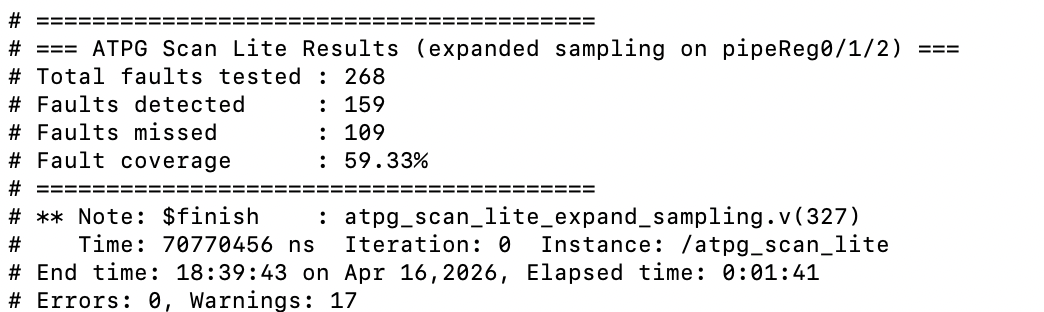
\includegraphics[width=0.8\linewidth]{figures/ATPG_sampl.png}
            \caption{Coverage with expanded scan bit sampling}
        \end{figure}
        
         \item \textbf{Multiple Iterations} I then applied multiple testing iterations to introduce additional pattern diversity.Coverage increases further, showing that repeated testing helps detect additional faults.
        
        \begin{figure}[h]
            \centering
            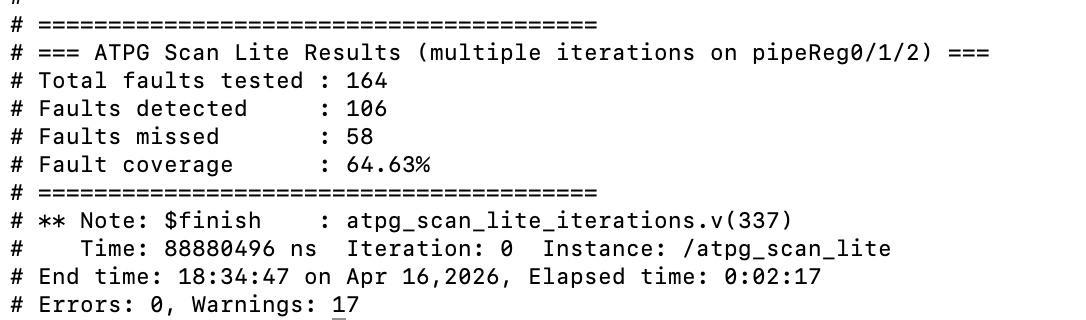
\includegraphics[width=0.8\linewidth]{figures/ATPG_iter.png}
            \caption{Coverage with multiple iterations}
        \end{figure}
        
        \item \textbf{Random Patterns} Finally, I applied diverse random patterns to improve fault excitation and propagation. This method achieves the highest coverage, indicating that pattern diversity plays an important role in improving test effectiveness.
        
        \begin{figure}[h]
            \centering
            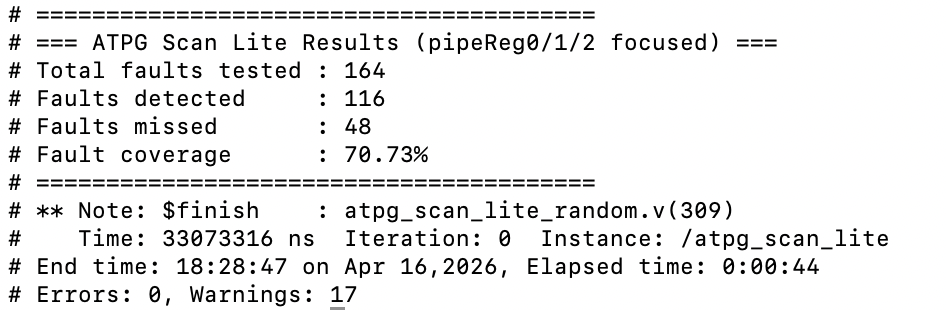
\includegraphics[width=0.8\linewidth]{figures/ATPG_random.png}
            \caption{Coverage with random patterns}
        \end{figure}
        
        The overall coverage improvement across different methods is summarized as follows. As shown, fault coverage increases from 52.31\% to 70.73\%, with random pattern generation providing the most significant improvement.
        
        \begin{figure}[h]
            \centering
            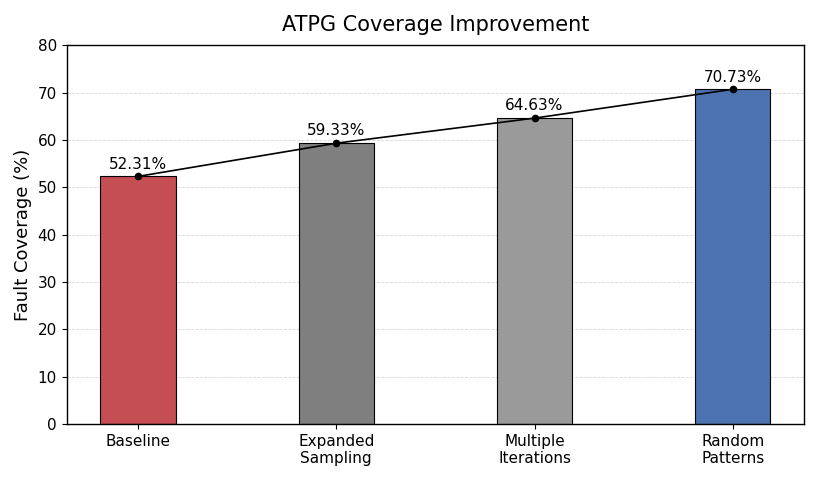
\includegraphics[width=0.9\linewidth]{figures/ATPG_cov.png}
            \caption{ATPG fault coverage across different methods}
        \end{figure}
        
        \end{itemize}
%%%%%%%%%%%%%%%%%%%%%%%%%%%%%%%%%%%%%%%%%%%%
    \subsection{Data Cache Verification Results}
        The verification environment successfully executed 200 constrained-random transactions and achieved full functional coverage of the targeted scenarios, including read hit/miss and write hit/miss behaviors. Both temporal locality (address reuse) and compulsory miss patterns were effectively exercised through the biased random stimulus strategy.
        
        In addition to functional coverage, the scoreboard-based checking mechanism enabled automatic validation of data correctness on a per-transaction basis. The monitor provided cycle-accurate traces, allowing detailed observation of DUT behavior during cache access and refill operations.
        
        During simulation, a consistent data mismatch was observed, revealing a functional bug in the RTL cache implementation. Specifically, in write-miss scenarios, an immediate read-back returned zero instead of the expected written value. This issue was reproducible and consistently affected addresses with a word offset of 7 within a cache block.
        
        Root-cause analysis traced the issue to the data cache interface module, specifically within the BURSTREAD state. The internal burst counter exhibited an off-by-one error, resulting in incorrect address sequencing during burst transfers. Consequently, the final word of the cache line was not properly loaded into the cache, leading to incorrect read-back data.
        
        The bug was systematically exposed by the constrained-random stimulus, particularly due to coverage of boundary offsets within a cache line. This demonstrates the effectiveness of the verification methodology in identifying non-trivial corner-case errors that may not be detected through directed testing alone.
%%%%%%%%%%%%%%%%%%%%%%%%%%%%%%%%%%%%%%%%%%%%
    \subsection{Verification Results (Core)}
        Coverage for the decoder and ALU was collected within the full core environment, allowing results to reflect realistic instruction flow rather than isolated module behavior. Instruction streams from an initial smoke test, along with additional RISCV-DV and targeted programs, propagated through the pipeline and exercised a wide range of execution paths. The initial test provided moderate coverage (~60\%) but left several instruction classes untested. By introducing targeted programs, coverage expanded to achieve 100\% across opcode, instruction type, and branch categories after merging all tests.
        
        ALU activity was driven through these same instruction streams, ensuring that operations were observed as part of normal datapath execution. The initial test primarily exercised arithmetic and comparison behavior (~60–70\% coverage), with limited diversity in operations. Additional programs introduced logical, shift, and varied operand-type instructions, resulting in near-complete coverage across the major ALU operation categories after merging.
        
        Cross coverage remained lower in comparison, as many combinations are not valid within the RV32I ISA and would require refinement to better reflect achievable scenarios.
        
        Overall, this approach ensures that coverage is representative of integrated processor behavior, capturing the interaction between decode and execute stages under realistic workloads.
%%%%%%%%%%%%%%%%%%%%%%%%%%%%%%%%%%%%%%%%%%%%%%%%%%%%%%%%%%%%%%%%%%%%%%%%%%%%%%%%%%
\section{Discussion}
%%%%%%%%%%%%%%%%%%%%%%%%%%%%%%%%%%%%%%%%%%%%
    \subsection{HYDRA RTL and Integration}
        Mode~A (scatter-gather) is the natural next addition: the descriptor 
        parser fits cleanly into the existing AGU and reuses the AHB master 
        FSM already validated for Modes~B and~C. Synthesis at 100~MHz in 
        130nm was deferred in favor of demonstrating correctness and measured 
        speedup pre- and post-DFF synthesis, consistent with how Wally itself 
        is validated and independent of any specific PDK. The scratchpad's 
        dual-port architecture and the ping-pong buffer both synthesize 
        cleanly from inferred DFFs, enabling post-synthesis verification 
        without requiring an SRAM macro library. The remaining critical 
        path is full SoC-level simulation: validating HYDRA's AHB master 
        under contention with the CPU's EBU and exercising the scratchpad's 
        dual-port behavior in the integrated bus fabric.
%%%%%%%%%%%%%%%%%%%%%%%%%%%%%%%%%%%%%%%%%%%%
    \subsection{Design for Testability (DFT)}
        Overall, this work establishes a complete scan-based DFT evaluation flow, from baseline coverage measurement to iterative improvement and root-cause analysis. Next semester, I plan to apply this methodology to our new design and explore more advanced DFT techniques to further improve test effectiveness.
%%%%%%%%%%%%%%%%%%%%%%%%%%%%%%%%%%%%%%%%%%%%
    \subsection{Data Cache Verification}
        The current verification framework establishes a functional UVM-based environment for cache validation, including a scoreboard and reference model for automated checking. Constrained-random stimulus and coverage-driven testing have been implemented to ensure sufficient exploration of cache behaviors.
        
        Future work will focus on extending test coverage to more complex scenarios, such as cache conflicts and boundary conditions, as well as improving debugging capability through additional assertions and enhanced observability.
%%%%%%%%%%%%%%%%%%%%%%%%%%%%%%%%%%%%%%%%%%%%
    \subsection{Core Verification}
        Further development should focus on expanding and refining covergroups within full-core simulations. While current covergroups capture decoder and ALU behavior, additional coverage can be introduced to target more complex pipeline interactions such as hazards, control flow behavior, and memory access patterns. Refining existing coverage (e.g., removing invalid cross combinations) will also improve the accuracy of reported metrics and better guide test development.
        
        Extending this framework to a more complex design such as the Wally processor does not require a fundamental change in structure, as both designs follow a similar 5-stage pipeline. However, Wally introduces significantly more complex interactions between stages, including more advanced hazard handling, control flow behavior, and inter-stage dependencies. To account for this, a more robust scoreboarding approach should be introduced. Integrating an architectural reference model (e.g., Spike) would enable comparison of full architectural state, including registers, memory updates, and control flow, providing stronger correctness checking beyond localized behavior.
        
        Supporting this transition will require enhancing the testbench to better observe and validate these interactions. This includes adding monitors for key pipeline stages, capturing stall and forwarding behavior, and tracking control flow events such as branch resolution and pipeline flushing. These additions allow the existing coverage-driven approach to scale into a more comprehensive system-level verification environment while maintaining the same overall methodology.
%%%%%%%%%%%%%%%%%%%%%%%%%%%%%%%%%%%%%%%%%%%%%%%%%%%%%%%%%%%%%%%%%%%%%%%%%%%%%%%%%%
\section{Acknowledgments}
    We would like to express our gratitude towards Professor Welsh and Professor Simar for their support of our project.
%%%%%%%%%%%%%%%%%%%%%%%%%%%%%%%%%%%%%%%%%%%%%%%%%%%%%%%%%%%%%%%%%%%%%%%%%%%%%%%%%%
\section{Credit Author Statement}
    \begin{itemize}
        \item \textbf{Nafil Atiq:} RTL review and core evaluation. %RTL design of RISC-V core.
        \item \textbf{Ruohan Dong:} UVM verification for RISC-V data cache.
        \item \textbf{Matthew Nutt:} RTL review and HYDRA architecture.
        \item \textbf{Giovanni Sirtori:} Literature review, HYDRA architecture, RTL implementation, and Wally SoC integration.
        \item \textbf{Ithzel Toscano:} UVM verification of RISC-V core.
        \item \textbf{Yulia Zhou:} Design for Testability (DFT).
    \end{itemize}
%%%%%%%%%%%%%%%%%%%%%%%%%%%%%%%%%%%%%%%%%%%%%%%%%%%%%%%%%%%%%%%%%%%%%%%%%%%%%%%%%%
\begin{thebibliography}{00}
    \bibitem{tripp2024}
    C.~E.~Tripp, J.~Perr-Sauer, J.~Gafur, A.~Nag, A.~Purkayastha,
    S.~Zisman, and E.~A.~Bensen, ``Measuring the energy consumption and
    efficiency of deep neural networks: An empirical analysis and design
    recommendations,'' arXiv:2403.08151, 2024.
    
    \bibitem{ti_edma}
    J.~Ward and J.~Bowen, ``TMS320C64x EDMA architecture,'' Texas
    Instruments Application Report SPRA994, Mar.\ 2004.

    \bibitem{harris2022wally}
    D.~Harris, S.~Stine, and M.~Thompson ``Wally: Configurable
    RISC-V processor,'' \textit{Harvey Mudd College}, 2022. [Online].
    Available: https://github.com/openhwgroup/cvw

    \bibitem{benz2023}
    T.~Benz, M.~Rogenmoser, P.~Scheffler, S.~Riedel, A.~Ottaviano,
    A.~Kurth, T.~Hoefler, and L.~Benini, ``A high-performance,
    energy-efficient modular DMA engine architecture,'' \textit{IEEE
    Transactions on Computers}, 2023, arXiv:2305.05240.
    
    \bibitem{ma2019}
    S.~Ma, Y.~Lei, L.~Huang, and Z.~Wang, ``MT-DMA: A DMA controller
    supporting efficient matrix transposition for digital signal
    processing,'' \textit{IEEE Access}, vol.~7, pp.~5808--5818, 2019.
\end{thebibliography}
\vspace{12pt}
%%%%%%%%%%%%%%%%%%%%%%%%%%%%%%%%%%%%%%%%%%%%%%%%%%%%%%%%%%%%%%%%%%%%%%%%%%%%%%%%%%

\end{document}